\documentclass[11pt]{article} % Default font size is 12pt, it can be changed here
\usepackage[french]{babel}
\usepackage{amsmath}
\usepackage{caption}
\usepackage{listings}
\lstset{literate=%
    {á}{{\'a}}1
    {é}{{\'e}}1
    {è}{{\`e}}1
    {í}{{\'i}}1
    {ó}{{\'o}}1
    {ú}{{\'u}}1
}
\lstset{
language=HTML,
basicstyle=\small,
lineskip={-1.5pt}
}
\usepackage[T1]{fontenc}
\usepackage[utf8]{inputenc}
\usepackage{geometry} % Required to change the page size to A4
\geometry{a4paper} % Set the page size to be A4 as opposed to the default US Letter

\usepackage{graphicx} % Required for including pictures

\usepackage{float} % Allows putting an [H] in \begin{figure} to specify the exact location of the figure
\usepackage{wrapfig} % Allows in-line images such as the example fish picture

\usepackage{lipsum} % Used for inserting dummy 'Lorem ipsum' text into the template

\usepackage{forest}

\usepackage{color}
\usepackage{multirow}


\linespread{1.2} % Line spacing

%\setlength\parindent{0pt} % Uncomment to remove all indentation from paragraphs

\graphicspath{{Pictures/}} % Specifies the directory where pictures are stored

% Add subsubsubsection
%\usepackage{titlesec}
%\setcounter{secnumdepth}{4}
%\titleformat{\paragraph}
%{\normalfont\normalsize\bfseries}{\theparagraph}{1em}{}
%\titlespacing*{\paragraph}
%{0pt}{3.25ex plus 1ex minus .2ex}{1.5ex plus .2ex}
%\setcounter{secnumdepth}{4}
%\setcounter{tocdepth}{4}

\begin{document}
%\newcommand{\citer}[1]{\footnotesize\par\noindent\textit{#1}\\}
\newcommand{\p}[1]{\par\noindent{#1}\\}
\newcommand{\pnr}[1]{\par\noindent{#1}}
\newcommand{\q}[1]{\par\noindent{\textbf{#1}}}
\newcommand{\m}[1]{\[#1\]}
\newcommand{\mt}[1]{$#1$}
\newcommand{\green}[1]{\textcolor{green}{#1}}

%----------------------------------------------------------------------------------------
%	TITLE PAGE
%----------------------------------------------------------------------------------------

\begin{titlepage}

\newcommand{\HRule}{\rule{\linewidth}{0.5mm}} % Defines a new command for the horizontal lines, change thickness here

\center % Center everything on the page

\textsc{\LARGE ESIEE Paris}\\[1.5cm] % Name of your university/college
\textsc{\Large PR-3602}\\[0.5cm] % Major heading such as course name
%\textsc{\large Projet}\\[0.5cm] % Minor heading such as course title

\HRule \\[0.4cm]
{ \huge \bfseries Résolution de problèmes en intelligence artificielle et optimisation
 combinatoire : les algorithmes A*} % Title of your document
\HRule \\[4cm]

\begin{minipage}{0.4\textwidth}
\begin{flushleft} \large
\emph{Auteurs:}\\
Boris \textsc{Ghidaglia}\\ % Your name
Augustin \textsc{Prolongeau}\\ % Your name
\end{flushleft}
\end{minipage}
~
\begin{minipage}{0.4\textwidth}
\begin{flushright} \large
\emph{Encadrant:} \\
M.\textsc{Couprie} % Supervisor's Name
\end{flushright}
\end{minipage}\\[4cm]

{\large \today}\\[3cm] % Date, change the \today to a set date if you want to be precise

{Sujet : https://perso.esiee.fr/~coupriem/PR3602/}

%\includegraphics{Logo}\\[1cm] % Include a department/university logo - this will require the graphicx package

\vfill % Fill the rest of the page with whitespace

\end{titlepage}

%----------------------------------------------------------------------------------------
%	TABLE OF CONTENTS
%----------------------------------------------------------------------------------------

\tableofcontents

\newpage

%----------------------------------------------------------------------------------------
%	Algorithme Naif
%----------------------------------------------------------------------------------------

\section{Algorithme naïf}

%------------------------------------------------
\subsection{Concept}
\p{Tester toutes les solutions possibles et choisir la moins couteuse.}

%------------------------------------------------
\subsection{Questions}
\q{Combien y'a-t il de solutions possibles ?}
\p{Le sujet stipule que nous sommes dans le cas d'une matrice \mt{N\times N}. Cela
signifie que chaque agent peut être attribué à N postes différents. Cependant, à chaque
 fois qu'un agent est affecté à un poste, c'est une combinaison en moins à tester pour
 tous les autres.  Ainsi, il y a \mt{N!} solutions possibles.}

\q{Si l'on suppose qu'une affectation peut être évaluée en une microseconde, et que l'on
 dispose de trois mois pour faire le calcul, quelle est la valeur maximum de \mt{N}
 possible pour envisager d'appliquer cette méthode ?}
\p{Calculons combien de microsecondes trois mois représentent (on considèrera qu'un
 mois dure environ \mt{30.5} jours) :}
\m{3\text{ mois} = 3\times 30.5\times 24\times 3600\times 10^6 = 7.9056\times 10^{12}\mu s}
\p{Il suffit alors de prendre la plus grande factorielle inférieure à cette valeur pour
 connaître notre \mt{N} maximal théorique :}
\m{16! = 2.0922789888\times 10^{13}}
\m{15! = 1.307674368\times 10^{12}}
\p{Notre \mt{N} maximum théorique est donc : \mt{15}. Si nous devons gérer une équipe
 de plus de 15 agents à affecter à plus de 15 postes, il nous sera impossible de calculer le
  résultat optimal via cet algorithme en trois mois ou moins.}



%----------------------------------------------------------------------------------------
%	Algorithme Glouton
%----------------------------------------------------------------------------------------
\newpage
\section{Algorithme glouton}

%------------------------------------------------
\subsection{Concept}
\p{Il s'agit de sélectionner la valeur minimale de la matrice des coûts, d'effectuer
 l'affectation correspondante et de retirer le poste et l'agent qui sont concernés, puis de
  recommencer jusqu'à affectation de la totalité de l'effectif.}

%------------------------------------------------
\subsection{Questions}
\q{Montrez par un contre-exemple simple que l'algorithme glouton ne trouve pas toujours
 la solution optimale pour ce problème}
\p{Posons les matrices $3\times 3$ suivantes: situation initiale, solution glouton et
solution optimale:}

\m{
\begin{bmatrix}
1 & 2 & 3 \\
2 & 4 & 5 \\
3 & 5 & 100
\end{bmatrix}
\begin{bmatrix}
\color{red}1 & 2 & 3 \\
2 & \color{red}4 & 5 \\
3 & 5 & \color{red}100
\end{bmatrix}
\begin{bmatrix}
1 & 2 & \color{green}3 \\
\color{green}2 & 4 & 5 \\
3 & \color{green}5 & 100
\end{bmatrix}
}\\

\p{On constate bien que l'algorithme glouton dévore la plus petite valeur de la matrice
 $C_{k}$ à chaque étape $k$, sans se soucier des conséquences de ses actes sur ses
  choix futurs.}

%----------------------------------------------------------------------------------------
%	Algorithme A*
%----------------------------------------------------------------------------------------
\newpage
\section{Algorithme A*}

%------------------------------------------------
\subsection{Avant d'aborder l'atelier : Test}
\q{Qu'est-ce qu'un Graphe de Résolution de Problème (GRP), relativement à un problème
 donné ?}
 \p{Un GRP est un graphe dont les sommets représentent les états possibles d'un problème donné.
  On peut passer d'un état $i$ à un état $j$ via un arc $u$ si une régle le permet.
   Cet arc se verra attribuer un coût $c(u)$. Le sommet initial représente l'état initial
    du problème et les sommets terminaux représentent chacun une solution possible du problème,
     ils se différencient principalement par le coût qui les séparent du sommet initial.}

\q{Quel GRP proposeriez-vous pour le problème de l'affectation ?}
\pnr{Il semble pertinent de représenter un arbre dans lequel chaque niveau $0,1,...,n$
 illustrerait l'affectation d'un poste $j$ appartenant à $0,1,...,n$, et chaque sommet serait
  un agent i appartenant à $0,1,...,n$ choisi. On ajoutera un coût $c$ sur chaque arc.
   Illustration avec $aX$ l'agent $X$, et sans représenter les coûts ni les numéros des
    postes (pour des raisons $LaTeXienne$) :}

\begin{align}
	\begin{forest}
	for tree={circle,draw, l sep=20pt}
	[Source
	    [a1
	      [a2
	        [a3]
	      ]
	      [a3
	        [a2]
	      ]
	    ]
	    [a2
	      [a1
	        [a3]
	      ]
	      [a3
	        [a1]
	      ]
	   ]
	   [a3
	     [a1
	       [a2]
	     ]
	     [a2
	       [a1]
	     ]
	   ]
	]
	\end{forest}
\end{align}
\newline

\newpage
\q{Quel est, schématiquement, le fonctionnement d'un algorithme A* ?}
\pnr{On pose : }

\begin{itemize}
  \item $OUVERT$ : une structure de données contenant les sommets découverts et non
   visités. On la maintiendra ordonnée par $f$.
  \item $FERME$ : une structure de données contenant les sommets visités.\\
\end{itemize}

\pnr{L'algorithme évolue schématiquement ainsi :}
\begin{itemize}
  \item Tant que $OUVERT$ non vide
  \item On récupère le meilleur sommet de la liste $OUVERT$, triée sur la base des valeurs
   de $f$ des sommets.
  \item \textbf{Si} ce sommet est un/l' objectif, $FIN$ : on retourne le chemin vers ce
  sommet en remontant les prédécesseurs. Ce chemin est optimal si $h \leq h*$
  \item \textbf{Sinon} on le place dans $FERME$ et on ajoute ses successeurs à $OUVERT$.\\
\end{itemize}

\q{Que représentent les symboles g, h et f dans l'algorithme ?}
\p{Dans l'algorithme, $g$ est la somme des coûts entre la source et un sommet $k$ via
 un chemin $c$. $h$ est une heuristique. Autrement dit, une estimation du coût entre ce
  sommet $k$ et un objectif $n$. Enfin : $f = g + h$}

\q{Quelle est la condition sur h pour que l'on parle d'algorithme A* ?}
\p{Pour que l'on parle d'algorithme $A^*$, on doit poser une heuristique $h$ telle que
 $h \leq h^*$, où $h^*$ est l'heuristique parfaite, l'estimation idéale.}

\newpage
%------------------------------------------------
\subsection{Heuristique nulle}

%------------------------------------------------
\subsubsection{Concept}
\p{L'heuristique nulle consiste simplement à attribuer une valeur $0$ aux $h$ de tous les
 sommets. L'algorithme se comporte alors comme celui de Dijkstra.}

%------------------------------------------------
\subsubsection{Preuve}
\p{On pose $C$ notre matrice de coûts, et $c$ un coût. $h_{0}$ l'heuristique nulle, $h^*$
 l'heuristique idéale.}

\begin{equation}
  \left.\begin{aligned}
  \forall c \in C, c \geq 0 \implies h^* \geq 0\\
  h_{0} = 0\\
\end{aligned}\right\}
\implies h_{0} \leq h^*
\end{equation}\\

%------------------------------------------------
\subsection{Somme des coûts minimums restants, par ligne}

%------------------------------------------------
\subsubsection{Concept}
\p{Il s'agit de sommer les coûts minimums d'affectation des jobs non encore affectés à
n'importe lequel des agents non encore affectés. Cette somme de minimums a été désignée
comme étant "par ligne", car si l'on se rapporte à notre arbre, chaque ligne
correspond en fait à un job.}

%------------------------------------------------
\subsubsection{Preuve}
\p{Comme nous l'avons compris grâce à l'arbre de la partie $3.1$, une affectation optimale
correspond au chemin de moindre coût joignant la source à une feuille. De plus, par définition
de cette heuristique, on peut affirmer qu'à tout moment de l'algorithme, la valeur $h$ estimée
par l'heuristique sera inférieure ou égale (cas où les valeurs minimums restantes à
chacune des lignes restantes peuvent exister dans une même combinaison d'affectations)
à la valeur de $h^*$.}

\newpage

\subsection{Somme des coûts minimums restants, par colonnes}

%------------------------------------------------
\subsubsection{Concept et Preuve}
\p{Même réflexion que pour l'heuristique : "Somme des coûts minimums restants, par ligne",
mais en parcourant pour chacun des agents non encore affectés leurs jobs non encore
affectés.}


\subsection{Maximum des valeurs des heuristiques par lignes et colonnes}

%------------------------------------------------
\subsubsection{Concept et intérêt}
\p{Le concept est simple : prendre la valeur maximum entre le résultat donné par
l'heuristique $3.3$ et $3.4$. Cela est intéressant car, $h^*$ étant l'heuristique parfaite, plus
on se rapproche de sa valeur, meilleure notre estimation est, et donc plus notre algorithme
sera efficace en général.}

\subsubsection{Preuve triviale}
\p{Posons $h_1$ l'heuristique $3.3$, $h_2$ l'heuristique $3.4$, $h$ l'heuristique
"Maximum des valeurs des heuristiques par lignes et colonnes" $h^*$ l'heuristique idéale.}

\begin{equation}
  \left.\begin{aligned}
  h_{1} \leq h^{*}\\
  h_{2} \leq h^{*}\\
\end{aligned}\right\}
\implies max(h_{1}, h_{2}) = h \leq h^*
\end{equation}\\
\newpage

\subsection{Minimum coefficienté}

%------------------------------------------------
\subsubsection{Concept}
\p{Contrairement à l'heuristique précédente qui est plus proche de $h^*$ que les $3.3$ et
$3.4$, celle-ci est plus éloignée, et donc moins efficace théoriquement. Son concept est
le suivant : on prend la valeur minimum parmi celles disponibles et on la multiplie par le
nombre d'affectations restant à effectuer (équivalent à la valeur que nous utilisons dans
le code : le nombre d'agents disponibles).}

\subsubsection{Preuve}
\p{Si l'on prend la valeur $v$ minimum parmi les valeurs disponibles et que l'on multiplie
celle-ci par le nombre d'étapes $p$ restantes, alors nous aurons nécessairement formé une
valeur inférieure ou égale à $h^*$. En effet, $h^*$ correspond à une somme de valeurs
différentes qui s'ajoutent à chaque étape. Or $v$ est la plus petite de toutes les valeurs
que $h^*$ pourrait être ammené à sommer. Ainsi, multiplier $v$ par $p$ donne nécessairement
une valeur inférieure à $h^*$. }

\newpage
%------------------------------------------------
\subsection{Performances}
\p{Dû à un problème de précision lié au calcul du temps d'exécution, nous avons créé une machine virtuelle Linux, le module python time étant plus précis sous Linux que sous Windows.}

\subsubsection{Matrice A}

\begin{center}
    \begin{tabular}{|c|c|c|c|}
        \hline
        \textbf{Heuristique} & \textbf{Exécution (s)} & \textbf{Noeuds visités} & \textbf{Ratio Visités/Total} \\ \hline
        Nulle &   0.00016   &  7   &  0.777 \\ \hline
        Min par ligne &   0.00027   &  5   &  0.555 \\ \hline
        Min par colonne &   0.00015   &  6   &  0.666 \\ \hline
        Max(lignes, colonnes) &   0.00016   &  5   &  0.555 \\ \hline
        Min coefficienté &   0.00014   &  6   &  0.666 \\ \hline
    \end{tabular}
\end{center}

\subsubsection{Matrice B}

\begin{center}
    \begin{tabular}{|c|c|c|c|}
        \hline
        \textbf{Heuristique} & \textbf{Exécution (s)} & \textbf{Noeuds visités} & \textbf{Ratio Visités/Total} \\ \hline
        Nulle &   0.00008   &  8   &  0.888 \\ \hline
        Min par ligne &   0.0001   &  6   &  0.666 \\ \hline
        Min par colonne &   0.00009   &  4   &  0.444 \\ \hline
        Max(lignes, colonnes) &   0.00018   &  4   &  0.444 \\ \hline
        Min coefficienté &   0.00011   &  6   &  0.666 \\ \hline
    \end{tabular}
\end{center}

\subsubsection{Matrice C}

\begin{center}
    \begin{tabular}{|c|c|c|c|}
        \hline
        \textbf{Heuristique} & \textbf{Exécution (s)} & \textbf{Noeuds visités} & \textbf{Ratio Visités/Total} \\ \hline
        Nulle &   0.00012   &  13   &  0.393 \\ \hline
        Min par ligne &   0.00030   &  7   &  0.212 \\ \hline
        Min par colonne &   0.00014   &  5   &  0.151 \\ \hline
        Max(lignes, colonnes) &   0.00024   &  5   &  0.151 \\ \hline
        Min coefficienté &   0.00027   &  8   &  0.242 \\ \hline
    \end{tabular}
\end{center}

\subsubsection{Matrice D}

\begin{center}
    \begin{tabular}{|c|c|c|c|}
        \hline
        \textbf{Heuristique} & \textbf{Exécution (s)} & \textbf{Noeuds visités} & \textbf{Ratio Visités/Total} \\ \hline
        Nulle &   0.00016   &  17   &  0.515 \\ \hline
        Min par ligne &   0.00017   &  5   &  0.151 \\ \hline
        Min par colonne &   0.00027   &  9   &  0.272 \\ \hline
        Max(lignes, colonnes) &   0.00030   &  5   &  0.151 \\ \hline
        Min coefficienté &   0.00035   &  12   &  0.363 \\ \hline
    \end{tabular}
\end{center}

\subsubsection{Matrice E}

\begin{center}
    \begin{tabular}{|c|c|c|c|}
        \hline
        \textbf{Heuristique} & \textbf{Exécution (s)} & \textbf{Noeuds visités} & \textbf{Ratio Visités/Total} \\ \hline
        Nulle &   33.4027   &  471337   &  5.018e-06 \\ \hline
        Min par ligne &   0.76576   &  854   &  9.092e-09 \\ \hline
        Min par colonne &   0.03716   &  65   &  6.920e-10 \\ \hline
        Max(lignes, colonnes) &   0.06729   &  60   &  6.387e-10 \\ \hline
        Min coefficienté &   20.1885   &  66813   &  7.113e-07 \\ \hline
    \end{tabular}
\end{center}

%----------------------------------------------------------------------------------------
%	Annexe
%----------------------------------------------------------------------------------------
\newpage

\section{Annexe}

\begin{figure}[!htb]
   \begin{minipage}{0.48\textwidth}
     \centering
     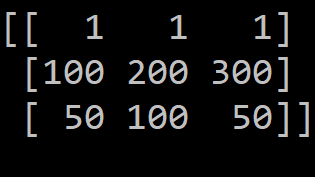
\includegraphics[width=.9\linewidth]{A.png}
     \caption{Matrice A}
   \end{minipage}\hfill
   \begin {minipage}{0.48\textwidth}
     \centering
     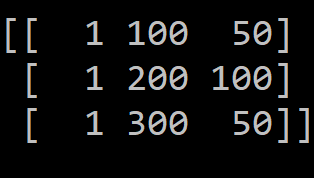
\includegraphics[width=.9\linewidth]{B.png}
     \caption{Matrice B}
   \end{minipage}
\end{figure}

\begin{figure}[!htb]
   \begin{minipage}{0.48\textwidth}
     \centering
     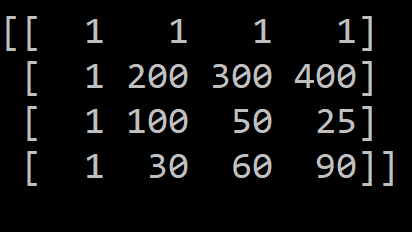
\includegraphics[width=.9\linewidth]{C.png}
     \caption{Matrice E}
   \end{minipage}\hfill
   \begin {minipage}{0.48\textwidth}
     \centering
     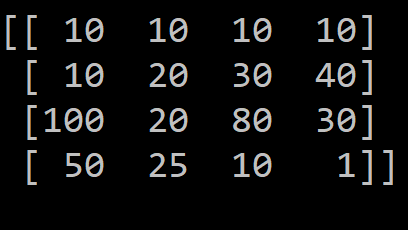
\includegraphics[width=.9\linewidth]{D.png}
     \caption{Matrice D}
   \end{minipage}
\end{figure}

\begin{figure}[!h]
  \begin{center}
    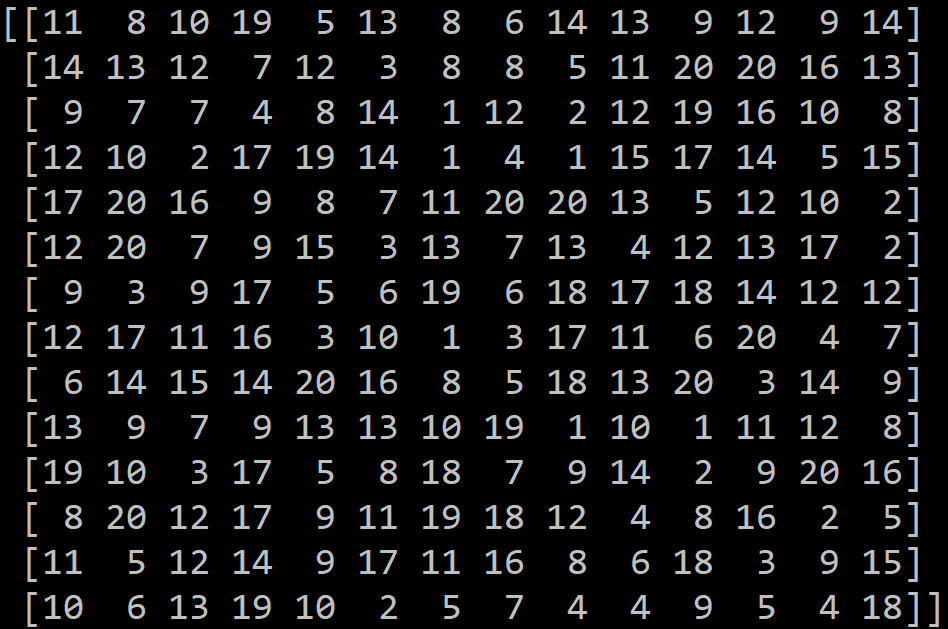
\includegraphics[width=.7\linewidth]{E.png}
    \caption{Matrice E}
  \end{center}
\end{figure}

\end{document}
